\chapter{Descrição da técnica}

A técnica usada neste trabalho é baseada em arestas e usa um modelo pré-definido para a pose inicial. A extração das arestas é feita por amostragem de pontos, descrita na seção anterior.

\begin{comment}
\section{Trabalhando com múltiplas hipóteses}

Um dos problemas que ocorrem nas técnicas \emph{edge-based} é que nem sempre se consegue extrair com precisão as arestas da imagem. Na seção anterior foi discutido que um dos passos para a extração das arestas é a procura por pontos de alto gradiente na normal da aresta. Muitas vezes é possível encontrar vários desses pontos para cada amostra, e neste caso obtém-se múltiplas hipóteses de pontos da imagem correspondente ao ponto amostrado. Veja a \figref{cubo_0}.

%O que se faz neste caso é, para cada aresta do modelo, trabalhar com múltiplos correspondentes na imagem.

%Como existem múltiplas hipóteses de correspondência em cada amostra do modelo, pode-se concluir que existirão múltiplas hipóteses de arestas para compor a pose da cena atual, como mostra a \figref{cubo_0}

O trabalho com múltiplas hipóteses foi inicialmente proposto em \cite{multiplas_hipoteses}. Neste trabalho cada aresta $E_i$ (do modelo) projetada na imagem tem um conjunto $\{e_{i,j}\}$ de pontos amostrados. Cada ponto $e_{i,j}$ tem um conjunto $\{e'_{i,j,l}\}$ de hipóteses de correspondência. Em \cite{multiplas_hipoteses} a hipótese $e'_{i,j,l}$ é aquela que tem a menor distância da aresta projetada $E_i$. Então mesmo que sejam encontrados pontos de forte gradiente na normal da aresta $E_i$, aquele que mais se aproxima da aresta projetada é escolhido como correspondente a $e_{i,j}$. Tendo este conjunto de correspondências, o processo continua como no caso de hipótese única.
\end{comment}

Na técnica de múltiplas hipóteses um dos candidatos é escolhido para ser associado com a amostra do modelo, no caso, o candidato mais próximo da aresta projetada. Entretanto isso nem sempre resulta na melhor pose final, pois outros pontos de forte gradiente, como objetos externos ou até uma outra aresta do próprio objeto, podem confundir todo o cálculo da pose só porque estão mais próximos de uma determinada aresta do modelo. Isso pode ser visualizado na \figref{multiplas_hipoteses_errada}, em que além da aresta do objeto, o lápis também é identificado pelo algoritmo de busca. O fato de uma das arestas do modelo projetado estar mais perto do lápis do que do próprio objeto faz com que o algoritmo de rastreamento o utilize como aresta do objeto e faça o cálculo de pose a partir disso, o que vai fazer uma grande diferença no processo de rastreamento a partir de então. Uma forma de contornar essa situação seria também escolher outras hipóteses (não somente a mais próxima) e calcular novas poses a partir de diferentes agrupamentos amostra-hipótese. O trabalho \cite{celine} propõe exatamente isso: que sejam calculadas diversas poses, utilizando hipóteses diferentes, para que no final as poses calculas sejam comparadas e a melhor dentre elas seja escolhida.

\begin{figure}[!ht]
\centering\includegraphics{monografia/multiplas_hipoteses_errada}
\caption{Casamento de hipóteses errado. O algoritmo encontrou múltiplas hipóteses para as amostras, mas optou por casar com as hipóteses erradas porque estavam mais próximas.}
\label{multiplas_hipoteses_errada}
\end{figure}

Um dos principais passos do algoritmo visa fazer combinações de agrupamento amostra-hipótese, pois combinar todos os possíveis casamentos amostra-hipótese não é uma estratégia válida, já que isso pode significar o cálculo de milhares de poses por cada \emph{frame}, mesmo que o objeto rastreado seja simples, como um cubo. Um outro problema de se fazer todas as possíveis combinações é que nem sempre um agrupamento de hipóteses revela uma possível aresta do objeto. Na \figref{agrupamento_errado_de_hipoteses} temos as amostras (em vermelho) e suas respectivas hipóteses (quadrados). A \figref{agrupamento_errado_de_hipoteses} exemplifica um caso de um casamento qualquer de amostras e hipóteses em que as hipóteses escolhidas estão em verde. A escolha dessas hipóteses claramente não resultaria em uma pose válida, pois o sistema iria tentar convergir uma de suas arestas (a com amostras vermelhas) para os pontos marcados em verde, e isso estaria longe de uma pose válida. Como o algoritmo trabalha com múltiplas hipóteses de pose, a pose gerada pela \figref{agrupamento_errado_de_hipoteses} provavelmente seria descartada em um passo posterior, mas é melhor evitar esse tipo de agrupamento para que sejam feitos menos cálculos de pose desnecessários. \cite{celine} sugere que se façam agrupamentos que sejam o mais próximo possível de uma reta, como exemplificado na \figref{agrupamento_certo_de_hipoteses}. Seguindo essa estratégia pode-se dizer que a abordagem trabalha não com múltiplas hipóteses de pontos do objeto, mas com múltiplas hipóteses de aresta. Veja a \figref{hipoteses_de_aresta}.

\begin{figure}[!ht]
\centering\includegraphics{monografia/agrupamento_errado_de_hipoteses}
\caption{Hipóteses agrupadas sem formar uma linha. Os pontos vermelhos são as amostras do modelo; os quadrados são as hipóteses de cada amostras; os quadrados de cor verde são as hipóteses escolhidas.}
\label{agrupamento_errado_de_hipoteses}
\end{figure}

\begin{figure}[!ht]
\centering\includegraphics{monografia/agrupamento_certo_de_hipoteses}
\caption{A figura mostra dois tipos agrupamentos (um rosa e outro verde) de modo que se aproximem de uma linha. Esse tipo de agrupamento é mais próximo de uma aresta que o mostrado na \figref{agrupamento_errado_de_hipoteses}}
\label{agrupamento_certo_de_hipoteses}
\end{figure}

\begin{figure}[!ht]
\centering\includegraphics{monografia/hipoteses_de_aresta}
\caption{A figura mostra dois tipos de agrupamento (um rosa e outro verde) formando duas hipóteses de aresta de mesma cor.}
\label{hipoteses_de_aresta}
\end{figure}

O uso de múltiplas hipóteses de aresta simplifica a escolha de hipóteses para se calcular novas poses. No caso, basta selecionar uma hipótese de aresta para cada aresta visível do modelo, que já é possível calcular uma nova pose. O critério para escolha da hipótese de aresta será discutido em breve, mas é importante ressaltar que apesar de todos os passos feitos até então, não se sabe com clareza quais das múltiplas hipóteses de aresta são arestas do objeto. É por isso que são feitas diferentes combinações dessas hipóteses para que diferentes poses sejam calculadas. O número de vezes em que hipóteses de arestas são escolhidas e novas poses são calculadas depende da quantidade de poses que se deseja obter. Depois de um número arbitrário de poses terem sido calculadas, o último passo é escolher uma pose dentre todas as poses calculadas. Cada pose possui um erro de reprojeção e o valor desse erro é o que vai ser usado para escolher a melhor pose.

Em poucas palavras o algoritmo se resume a:

\begin{itemize}
	\item Projetar o modelo usando a pose do quadro anterior;
	\item Amostrar as arestas do modelo projetado;
	\item Fazer uma busca por pontos de forte gradiente na normal de cada amostra. Esses pontos serão as hipóteses da amostra;
	\item Em cada aresta, criar grupos de hipóteses de modo que não existam duas hipóteses em um mesmo grupo que pertençam à mesma amostra. Esses grupos devem aproximar, da melhor forma possível, seus elementos de uma reta;
	\item Para cada aresta visível do modelo, escolher uma de suas hipóteses de aresta e calcular a pose que projeta o modelo o mais próximo possível das arestas selecionadas. Observe que a escolha das hipóteses de aresta seguido do cálculo da pose se assemelha bastante à técnica de extração explícita de aresta, visto na seção \ref{sec:extracao_explicita};
	\item Repetir o passo anterior tantas vezes quanto forem a quantidade de poses necessárias;
	\item Avaliar o erro de cada pose calculada e escolher a que possuir o menor erro de reprojeção.
\end{itemize}

\section{Extraindo a hipótese de aresta}

Uma das primeiras etapas do algoritmo é o agrupamento das hipóteses de cada amostra em conjuntos cujos elementos formam uma reta (ou o mais próximo disso). Vale ressaltar que o processo de extração dessas hipóteses é pela amostragem de pontos, descrito em detalhes na seção \ref{sec:amostragem_de_pontos}.

As hipóteses de aresta são formadas agrupando $k_i$ conjuntos de $e'_{i,j,l}$. Cada aresta $E_i$ do modelo possui um conjunto $\{e_{i,j}\}$ de amostras (veja a seção \ref{sec:amostragem_de_pontos}) e cada uma dessas amostras está associada a um conjunto de hipóteses $\{e'_{i,j,l}\}$, como mostra a \figref{multiplas_hipoteses_celine}. O número $k_i$ de conjuntos é dado pelo maior número de hipóteses detectadas por uma amostra da aresta $E_i$, ou seja $k_i = max_j\{n_{i,j}\}$, sendo $n_{i,j}$ o número de candidatos associados à amostra $e_{i,j}$.

\begin{figure}[!ht]
\centering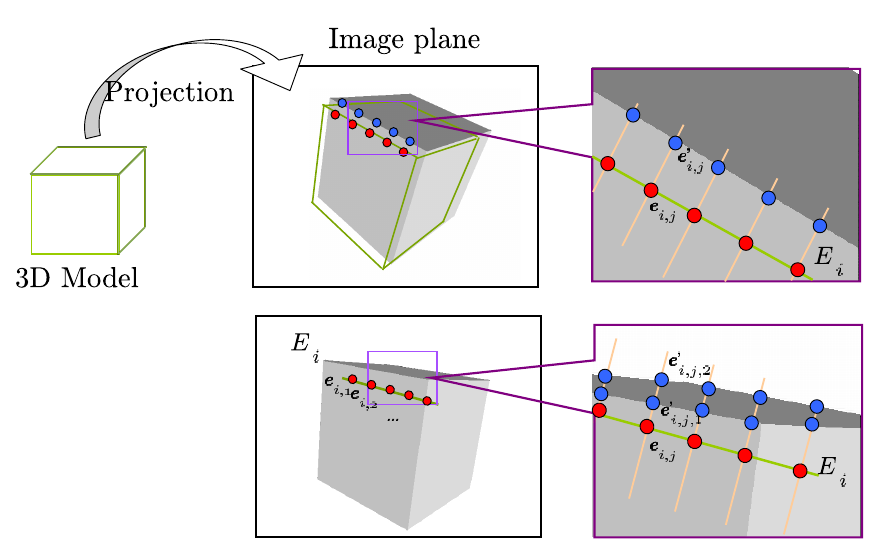
\includegraphics[width=0.9\textwidth]{monografia/multiplas_hipoteses_celine}
\caption{Visualização das múltiplas hipóteses. Figura retirada de \cite{celine}.}
\label{multiplas_hipoteses_celine}
\end{figure}

O agrupamento dessas hipóteses é feito utilizando o algoritmo de classificação \emph{k-means}. A classificação tem a tarefa de decidir a que grupo cada hipótese vai pertencer. Como o objetivo é que o conjunto de pontos de cada grupo (ou classe) sejam o mais colineares possíveis, esta etapa deve alocar as hipóteses para cada grupo de forma que cada novo elemento adicionado contribua com a colinearidade do grupo. Seja $\{e'_{i,j,l}\}$ o conjunto de elementos da aresta $E_i$, o objetivo é distribui-los entre as $k_i$ classes de $E_i$, definidas por $(c^i_1, \dots, c^i_{k_i})$.

% TODO: aqui já se sabe que cada aresta trabalha de forma independente. thread nelas!

%Para formar esses conjuntos, as hipóteses $e'_{i,j,l}$ de cada amostra são agrupadas utilizando um algoritmo de classificação \emph{k-means}. Para cada aresta $E_i$, o algoritmo agrupa as hipóteses de pontos $e'_{i,j,l}$ em $k_i$ conjuntos (ou classes), que será chamada de $(c^i_1, \dots, c^i_{k_i})$. O centróide de cada classe é a reta resultante do algoritmo \emph{fitline} \cite{fitline_doc} com o conjunto de pontos da classe.

Inicialmente as hipóteses $e'_{i,j,l}$ da aresta $E_i$ são agrupadas nas classes $(c^i_1, \dots, c^i_{k_i})$ na ordem em que elas foram encontradas na busca pela normal. Dessa forma a classe $c^i_m$ é formada inicialmente pelo conjunto $\{e'_{i,j,m}\}$, em que $0 < j \leq n_i$ e $n_i$ é o número de amostras da aresta $E_i$. Em outras palavra, as hipóteses mais próximas das amostras serão colocadas nas primeiras classes. Esse é um bom agrupamento inicial, já que boa parte das amostras já estão localizadas no seu \emph{cluster} final.

Em seguida ocorre o procedimento iterativo de reagrupar as hipóteses. Nessa etapa, o primeiro passo é computar o centróide de cada classe. O centróide é uma reta do espaço cuja soma das distâncias de cada elemento da classe para a reta é a menor possível. A estimativa dessa reta é calculada através de um procedimento denominado \emph{fitline} \cite{fitline_doc}. O que ele faz basicamente é encontrar uma reta que minimiza o erro (definido pela soma das distâncias de cada elemento da classe à reta) de cada \emph{cluster}.

Para cada amostra $e_{i,j}$ é executado outro procedimento iterativo que reagrupa as hipóteses nos \emph{clusters}. Nessa etapa é calculada a distância das hipóteses $\{e'_{i,j,l}\}$ da amostra $e_{i,j}$ para todos os centróides. Isso é feito para que a hipótese seja movida para o \emph{cluster} cujo centróide seja o mais próximo. Porém pode acontecer de mais de uma hipótese da mesma amostra ter o mesmo \emph{cluster} como o mais próximo, mas infelizmente somente uma delas pode ir para o \emph{cluster}, pois como foi visto, não podem existir duas hipóteses de uma mesma amostra em uma mesma classe. A solução para isso foi definir que o primeira hipótese teria prioridade sobre as hipóteses seguintes, ou seja, quando uma hipótese tiver sido movida para uma classe, nenhuma das outras hipóteses seguintes que serão avaliadas poderão optar pela mesma classe. Quando ocorrer da hipótese optar por uma classe que já tiver sido ocupada, ela será movida para o segundo \emph{cluster} mais próximo. Devido a isso, ao invés do cálculo das distâncias guardar apenas o centróide mais próximo da hipótese, nessa etapa cada hipótese mantém uma lista com os centróides ordenados por ordem de distância. Assim fica mais fácil de saber qual o segundo (ou terceiro) centróide mais próximo quando se tenta alocar a hipótese a um \emph{cluster} já ocupado.

% TODO: fazer algoritmo, pseudocodigo

No trabalho original \cite{celine} é dito que esse último passo seja repetido até que não haja mais trocas entre as classes, mas na prática precisou-se estabelecer um número máximo de iterações, pois muitas vezes o algoritmo repetia indefinidamente.

% TODO: Esses passos são melhor explicados no algoritmo abaixo.

Ao final das iterações é computado o erro residual $r^i_m$, de cada classe $c^i_m$. O erro residual é calculado pela média das distâncias de cada elemento da classe para o seu centróide. Ele indica o quão próximo de uma reta o conjunto de elementos da classe está, como mostra a equação

\begin{equation}
r^i_m = \frac{1}{N} \sum^{N}_{j = 0} \text{dist} (e'_{i,j,m}, c^i_m)
\end{equation}

em que $N$ é o número de elementos do \emph{cluster} $c^i_m$, e $\text{dist} (e', c)$ é a função que calcula a distância do ponto $e'$ à reta $c$. O resíduo $r^i_m$ será usado na próxima seção e influenciará na escolha das hipóteses de aresta.

\section{Obtendo as hipóteses de pose}

As hipóteses de pose são calculadas a partir de um conjunto de hipóteses de aresta selecionadas. Nesse ponto não é fácil avaliar quais das hipóteses de aresta são as mais corretas, por isso que elas são combinadas de formas diferentes de modo que sejam calculadas várias poses. Portanto é razoável que em cada combinação as hipóteses de aresta sejam escolhidas aleatoriamente. Entretanto cada hipótese tem um erro residual $r^i_m$ associado, e apesar desse erro não indicar necessariamente que uma determinada hipótese é uma boa escolha, ele pode pelo menos ajudar na escolha da aresta. É por isso que apesar da escolha ser aleatória, cada hipótese de aresta $c^i_m$ tem um peso $w^i_m$ que o ajuda a ser sorteado. O peso $w^i_m$ é dado pela equação \cite{celine}

\begin{equation}
w^i_m = \begin{cases}
    e^{-\lambda \left( \frac{r^i_m - r^i_{min}}{r^i_{max} - r^i_{min}}\right)^2 } & \mbox{se } r^i_{max} \neq r^i_{min} \\
    1 & \mbox{senão}.
\end{cases}
\end{equation}

em que $\lambda$ é um parâmetro que pode ser ajustado.

Mesmo tendo calculado os pesos, é importante fazer uma escolha aleatória porque pode ser que alguma hipótese, mesmo tendo o menor peso, seja a melhor escolha para a pose do quadro atual. Por outro lado vale a pena se utilizar dos pesos (e não somente escolher uma hipótese ao acaso) porque o fato de um \emph{cluster} ser formado por pontos que se aproximam bastante de uma reta já dá um indício (menos não sendo tão forte) que determinada hipótese pode ser uma boa escolha.

% TODO A escolha aleatória com pesos é equivalente a girar uma roleta em que determinadas casas são maiores que outras (como mostra a \figref{random_weighted_choice}). O algoritmo usado pode ser visto no pseudocódigo abaixo.

% TODO algoritmo da escolha aleatoria com pesos

Após isso é calculado o erro de reprojeção de cada pose formada. A que possuir menor erro é considerada a pose da cena atual e será usada para as próximas iterações do algoritmo.

\section{Uso da GPU}

Neste trabalho de graduação a técnica foi implementada tanto em C++ quanto em CUDA, plataforma de computação paralela criada pela NVIDIA que compila código para ser executado na GPU. A decisão de se implementar para essa plataforma foi feita após avaliar que o algoritmo era computacionalmente complexo, mas com cálculos bastante independentes, o que é um excelente caso para implementar um algoritmo que seja executado em paralelo. As placas atuais da NVIDIA possuem várias unidades de processamento que, apesar de serem individualmente mais lentas que uma CPU atual, tem a vantagem de se comunicar rapidamente entre seus outros \emph{cores}.

As placas da NVIDIA que suportam CUDA agrupam suas unidades de processamento em blocos e cada bloco, por sua vez, possui várias \emph{threads} (veja a \figref{cuda_grid}). Diferentes \emph{threads} podem trocar mensagens entre si através da memória compartilhada, contanto que elas estejam no mesmo bloco. Se estiverem em blocos diferentes elas podem se comunicar através da memória global, porém esse tipo de comunicação é mais lento. Veja o diagrama da \figref{cuda_memory}.

Na etapa de classificação do algoritmo apresentado, pode-se observar que cada aresta $E_i$ trabalha de forma independente umas das outras. Nenhum tipo de cálculo feito em uma aresta interfere no resultado de outra. Isso já é um bom indício que a clusterização utilizando o \emph{k-means} pode ser executados em diferentes \emph{threads}.

\textbf{FAZER:}
\begin{itemize}
	\item falar que as amostras também podem ficar em threads separadas
	\item o fitline também pode ser executado em threads separadas (ver como foi a logica que usei)
	\item falar que há um limite de threads por bloco. por isso que não bota todas as arestas em um bloco só. tem que separar as arestas por bloco.
	\item fitline teve que ser reimplementado em GPU. o código foi baseado no código do OpenCV, mas a licença deles permite.
\end{itemize}

\begin{figure}[t]
\centering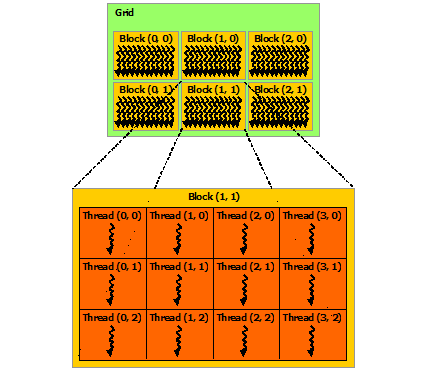
\includegraphics{monografia/cuda_grid}
\caption{Esquema de separação de blocos e \emph{threads} das placas da NVIDIA}
\label{cuda_grid}
\end{figure}

\begin{figure}[t]
\centering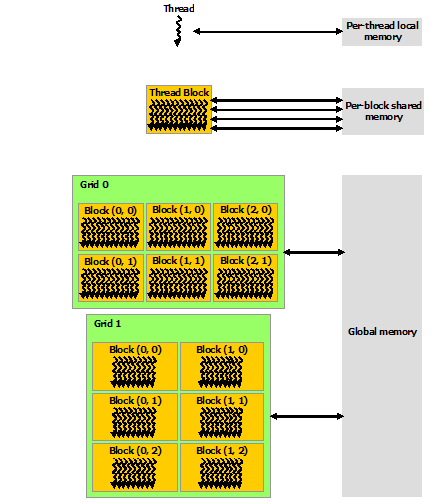
\includegraphics{monografia/cuda_memory}
\caption{Organização de memória das placas da NVIDIA}
\label{cuda_memory}
\end{figure}

% por que usar?
%% o algoritmos é lento
% dá pra usar?
%% sim, porque chega uma hora que é cada um por si :) dá para colocar várias coisinhas em threads diferentes
% por que GPU é bom? o que ela faz demais?
%% muitos cores para realizar continhas
% desvantagens?
%% branch do código? ("if")

\begin{comment}
\section{Rascunho}

\begin{figure}[ht!]
\centering
\includegraphics{monografia/cubo_arestas}
\caption{}
\label{cubo_arestas}
\end{figure}

A \figref{cubo_arestas} ilustra que as hipóteses de aresta são extraídas a partir das hipóteses das amostras. A escolha das arestas foi feita de maneira que para cada amostra escolhida, a primeira hipótese encontrada irá compor a primeira aresta; a segunda hipótese fará parte da segunda aresta e assim por diante.

\begin{figure}[ht!]
\centering
\includegraphics{monografia/cubo_kmeans}
\caption{}
\label{cubo_kmeans}
\end{figure}

No algoritmo usado nesse trabalho, baseado em \cite{celine}, é feita uma clusterização usando \emph{k-means} para que as hipóteses fiquem o mais próximo possível das arestas formadas. Como ilustrado na \figref{cubo_kmeans}, as hipóteses da \figref{cubo_arestas} são realocadas para que cada conjunto hipóteses forme um \emph{cluster} (ou aresta).

\section{Escolha da pose}

Para cada aresta da pose anterior, uma das hipóteses de aresta é escolhida aleatoriamente e assim será formada a pose atual.
\end{comment}

\begin{comment}
\section{A FAZER}

\begin{enumerate}
\item Descrever o moving-edges. Mostrar que com múltiplas hipóteses a $n$-ésima hipótese de ponto vai corresponder à $n$-ésima hipótese de aresta.
\item Falar sobre \cite{celine}. As hipóteses de pontos vão formar arestas tal que elas fiquem as mais paralelas possíveis da aresta da cena atual.
\item colocar figuras para ilustrar
\end{enumerate}
\end{comment}
